\documentclass{beamer}
\usepackage{beamerthemesplit}
\usepackage{graphics}
\logo{
\includegraphics[height=1cm]{psi_logo_white.png}}
\usetheme{Pittsburgh}
\usecolortheme{dove}
\beamertemplatenavigationsymbolsempty
\setbeamertemplate{footline}[frame number]
\definecolor{myback}{RGB}{175,238,238}
\setbeamercolor{structure}{bg=myback}
\usepackage[T1]{fontenc}
\newcommand{\changefont}[3] {
 \fontfamily{#1} \fontseries{#2} \fontshape{#3} \selectfont}

\title{The NeXus Data Format for muon Spectroscopy and Neutron or X-ray Scattering }
\author{Mark K\"onnecke }
\institute{Paul Scherrer Institute\\Switzerland }
\date{\today} 

\begin{document}

\begin{frame}
\titlepage
\end{frame}

\begin{frame}
\frametitle{The Predicament of the Traveling Scientist}
\begin{itemize}
\item<1->A different data format wherever she goes
\item<2->Spends lots of time converting formats or writing readers
\item<3->Waits even longer to load data from inefficient data formats
\item<4->DA requires N files in different  formats, notes, local knowledge 
\item<5->Cannot read her collaborators data
\item<6->Has to keep extra information in yet another form
\end{itemize}
\end{frame}

\begin{frame} \frametitle{NeXus Design}
\begin{itemize}
\item Complete data for typical use
\item Extendable, add additional data as you please
\item Self describing
\item Easy automatic plotting
\item Platform independent, public domain, efficient
\item Suitable for a wild variety of applications
\end{itemize}
\end{frame}

\begin{frame} \frametitle{NeXus History }
\begin{itemize}
\item Devised from three independent proposals by Jonathan Tischler, 
  APS, Przemek Klosowski, NIST and 
 Mark Koennecke, ISIS, PSI in 94-96
\item Improved during various NOBUGS conferences
\item NeXus International Advisory Committee, NIAC, since 2003
\item Since 2003 yearly meetings of the NIAC
\item We already considered many issues!
\item Except for one year, we never had money to develop NeXus
\end{itemize}
\end{frame}

\begin{frame}
 \frametitle{NeXus Levels }
\begin{enumerate}
\item Physical file format and API for accessing files
\item Rules for storing data in files
\item Component and application definitions
\item NeXus Utilities
\end{enumerate}
\end{frame}


\begin{frame} \frametitle{Physical File Format }
\begin{itemize}
\item Portable, self describing, extendable, public domain
\item Hierarchical data format, NCSA, HDF-4, later HDF-5
\item HDF-5:
\begin{itemize}
\item grouping support
\item on the fly compression
\item reading/writing subsets
\item first dimension appendable
\item Public domain C, F77 access library
\item Used by: NASA, Boing, the weathermen, .... 
\end{itemize}
\item XML for those who wish to edit their data
\end{itemize}
\end{frame}


\begin{frame} \frametitle{NeXus API }
\begin{itemize}
\item NeXus-API hides complex HDF API
\item Transparent access to all three supported physical file formats
\item ANSI-C implementation
\item Bindings: C++, F77, Java, python, IDL, SWIG
\item January, 4, 2010: 1311217 files processed at PSI alone
\end{itemize}
\end{frame}


\begin{frame}[fragile]
 \frametitle{NeXus API Example }
\begin{semiverbatim}
nxfile = nxs.open('hrpt2008n152088.hdf','r')
nxfile.openpath('/entry1/data1/two_theta')
x = nxfile.getdata()
nxfile.openpath('/entry1/data1/counts')
y = nxfile.getdata()
nxfile.openpath('/entry1/title')
txt = nxfile.getdata()
nxfile.close()

plot(x,y)
xlabel('two theta')
ylabel('counts')
title(txt)
show()
\end{semiverbatim}
\end{frame}

\begin{frame} \frametitle{NeXus Objects}
\begin{itemize}
\item Files
\item Groups identified by name and a classname beginning with NX
\item Scientific data sets
\item Attributes
\item Links
\end{itemize}
\end{frame}

\begin{frame} \frametitle{Rules for Storing Data in NeXus Files}
\begin{itemize}
\item NeXus files have a hierarchy
\item NXentry
\begin{itemize}\item NXuser
\item NXsample
\item NXmonitor
\item NXdata
\item NXinstrument
\begin{itemize}\item NXmonochromator
\item NXdetector
\item ...
\end{itemize}\end{itemize}
\end{itemize}
\end{frame}

\begin{frame} \frametitle{Why the Hierarchy??}
\begin{itemize}
\item<1->Supports self description and allows short names in components
\item<2->Name, classname pair allows for multiple components of the same type
\item<3->NXentry allows for multiple datasets in the same file
\item<4->NXdata supports automatic plotting
\item<5->Take care once when writing, use n times
\end{itemize}
\end{frame}


\begin{frame} \frametitle{Storing Single Data Items }
\begin{itemize}
\item Units have to specified
\item Locating axis, by example
\item (Proposed) Taking care of scaled data
\end{itemize}
\end{frame}



\begin{frame} \frametitle{NeXus Component and Application Definitions }
\begin{itemize}
\item Component definitions: 
 dictionaries of allowed field names for the various NeXus groups
{\changefont{cmr}{bx}{sc} 
\item Application Definitions
\begin{itemize}
\item Define what has to be in a NeXus file for a certain application
\item Defines standards
\item Another view: Contract between file producers and users about what has to be in 
 a NeXus file for a well defined purpose 
\item Validation by NXvalidate
\end{itemize}
}
\item Written in NeXus Definition Language, NXDL
\end{itemize}
\end{frame}

\begin{frame} \frametitle{Available NeXus Application Definitions}
{\changefont{cmr}{bx}{sc} 
\begin{tabular}{lll}
NXarchive& NXmonopd & NXrefscan \\
NXreftof & NXsas & NXscan \\
NXtas & NXtofraw& NXtomo\\
NXtomophase & NXxeuler & NXxkappa\\
NXxnb & NXxrot & NXiqproc \\
NXtomoproc & NXtofsingle& \\
\end{tabular}
}
\end{frame}


\begin{frame} \frametitle{Application Definition Process}
\begin{enumerate}
\item Construct an application definition with advice from the NIAC
\item Cure for a year; data should be produced in the new format in this time
\item After curation and review: this is the standard for this application type.
\end{enumerate}
\begin{itemize}
\item No promises, but the NIAC may do it for you
\begin{itemize}
\item Description of experiment
\item Minimum set of data items necessary form common use
\item Example data
\end{itemize}
\end{itemize}

\end{frame}


\begin{frame} \frametitle{NeXus Tools}
\begin{description}
\item[nxbrowse] CLI NeXus browser
\item[nxtree] prints NeXus tree
\item[NXmeta] dumps all NeXus meta data
\item[nxtranslate] transforms into NeXus 
\item[nxvalid] validates NeXus files 
\item[nxextract] converts from neXus to ASCII and binary
\item[nxplot] plots any NeXus file
\end{description}
\end{frame}

\begin{frame} \frametitle{NeXus Conversions}
\begin{figure}[!ht]
\resizebox{7cm}{5cm}{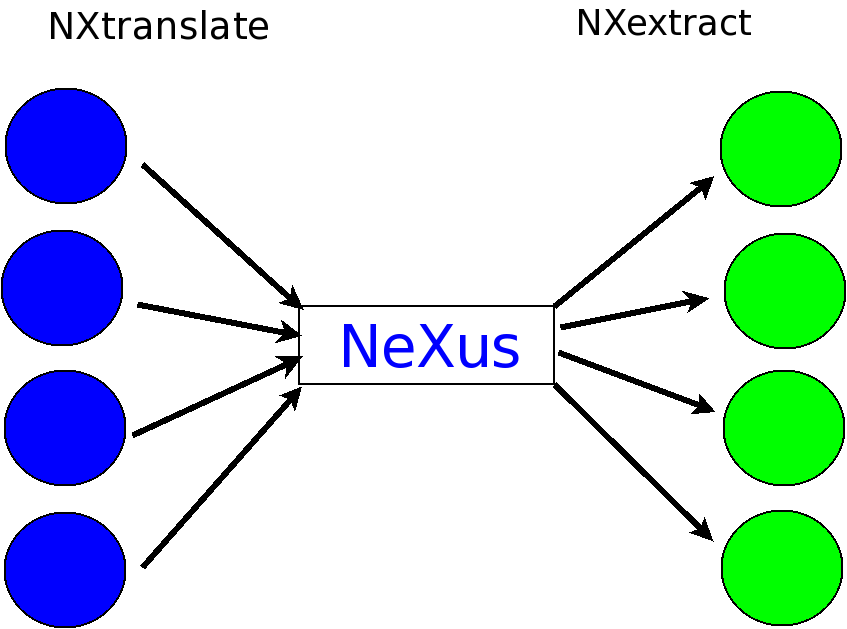
\includegraphics[width=0.75\textwidth]{nxswarch.png}}
\end{figure}
\end{frame}


\begin{frame} \frametitle{NXplot }
\begin{figure}[!ht]
\resizebox{7cm}{5cm}{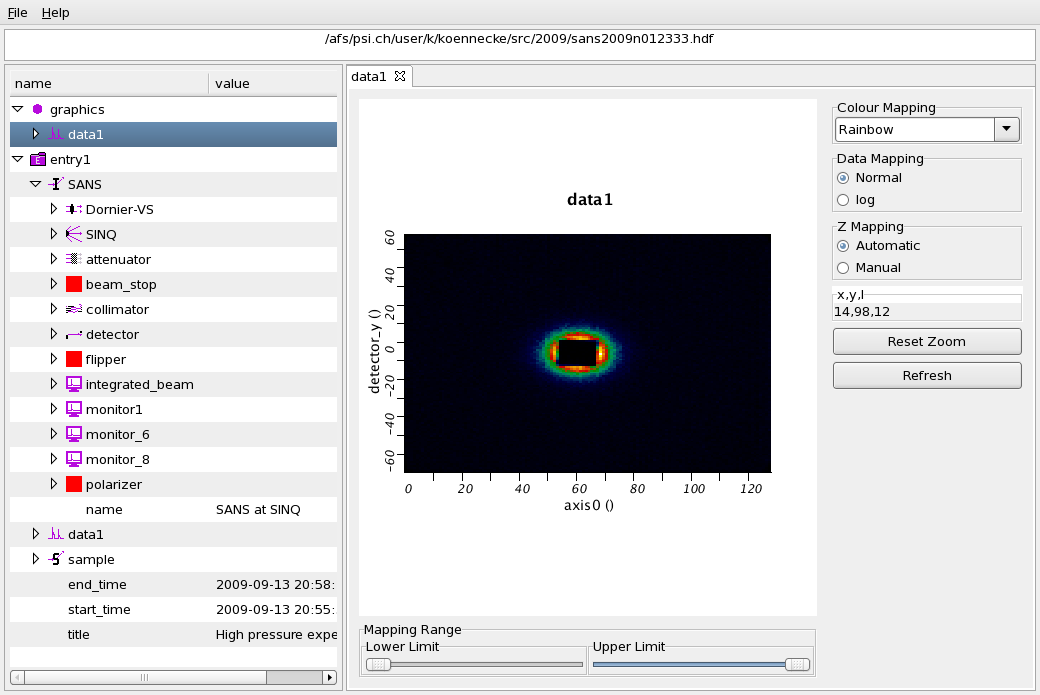
\includegraphics[width=0.75\textwidth]{NXplot.png}}\end{figure}
\end{frame}

\begin{frame} \frametitle{Other Systems Using NeXus}
\begin{itemize}
\item DANSE
\item DAVE
\item FABLE (ESRF)
\item ISAW
\item LAMP
\item openGenie
\item ICAT
\item Mantid
\item openGDA
\item All HDF tools
\end{itemize}
\end{frame}

\begin{frame} \frametitle{Data Format Challenges}
\begin{description}
\item<1->[Challenge 1] in science you are supposed to do new, non standard, things.  
 These of course cannot be easily cast into a standard.
\item<2->[Challenge 2] in order to establish a standard a lot of people need to agree
\item<3->[Challenge 3] a standard requires scarce scientific  programming resources for adoption 
\end{description}
\end{frame}

\begin{frame} \frametitle{Data Format Chances}
\begin{description}
\item<1->[Chance 1] By using a discoverable data format like NeXus, XML, HDF-5, people can at 
 least figure out  what is in the data file. 
\item<2->[Chance 2] Using predefined names from a dictionary gives meaning to the data in a file.
\item<3->[Chance 3] Using a shared API reduces learning costs and increases application stability.
\item<4->[Chance 4] With NeXus, HDF-5 plus professional programming techniques a DA application can 
 read any file which contains the required data.
\item<5->[Chance 5] Storing as much data as possible increases the likelihood that the needed 
 data is actually on file, even for unforeseen uses. 
\item<6->[Chance 6] In many experiments not the technique but the sample is important: 
 then an application definition simplifies life.  
\end{description}
\end{frame}


\begin{frame} \frametitle{Who commits to NeXus? }
\begin{figure}[!ht]
\resizebox{7cm}{5cm}{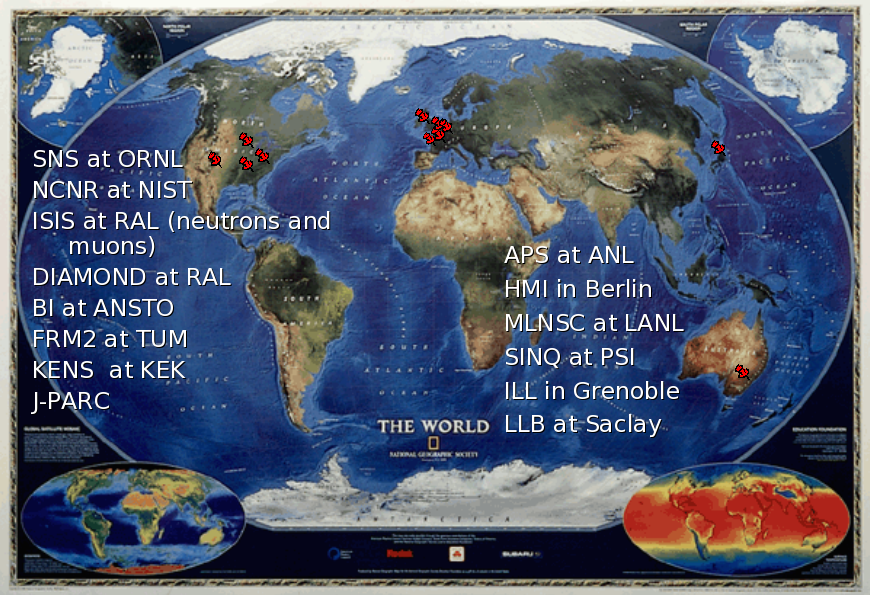
\includegraphics[width=0.75\textwidth]{nxworld.png}}\end{figure}
\end{frame}

\begin{frame} \frametitle{What You Can Do with NeXus}
\begin{enumerate}
\item Store and archive data from a wild variety of instruments
\item Store processed data
\item Store a complete workflow from raw data to publication ready data in several 
 NXentries in one file
\item Store a set of related experiments in one file
\item Define strict and validatable standards 
\end{enumerate}
\end{frame}

\begin{frame} \frametitle{Aims of this Workshop }
\begin{itemize}
\item Disseminate detailed Information about NeXus and NAPI
\item Add synchrotron specific data fileds and base classes to NeXus
\item Create a synchrotron wishlist for the NIAC
\item Create application definitions for synchrotron specific instrumentation
\item Review existing application definitions 
\item http://www.nexusformat.org
\item http://lns00.psi.ch/nexus2010
\end{itemize}
\end{frame}



\end{document}

\begin{frame} \frametitle{Conclusion }
\begin{itemize}
\item NeXus is a mature and capable data format
\item There is no other standard then NeXus on the horizon
\item New things are developed with NeXus everywhere, uptake at established sites is slow
\item You are invited to join the NIAC and contribute to NeXus 
\item More information: http://www.nexusformat.org (outdated, but working on it)
\end{itemize}
\end{frame}


\begin{frame} \frametitle{Example Files}
\end{frame}

\begin{frame} \frametitle{Storing Single Data Items }
\begin{itemize}\item Units have to specified
\item Locating axis, by example:
\begin{itemize}\item counts(two\_theta, time\_of\_flight), attributes: signal=1
\item two\_theta, attributes: axis=1, axis=primary 
\item time\_of\_fligth, attributes: axis=2, axis=primary
\end{itemize}\end{itemize}
\end{frame}

\begin{frame} \frametitle{NXtranslate }
\begin{itemize}\item Anything to NeXus converter:
\begin{itemize}\item Binary dump
\item FRM2
\item IPNS run
\item NeXus
\item Spec
\item XML
\end{itemize}\item Uses XML based translation file to control translation
\item Extendable via plugins
\end{itemize}
\end{frame}

\begin{frame} \frametitle{NXextract}
\begin{itemize}
\item Extracts NeXus files to binary or ASCII
\item Uses XML template file to control conversion
\item Contributed by Stephane Poirier, SOLEIL 
\end{itemize}
\end{frame}

\begin{frame} \frametitle{Another Way to use NeXus/HDF-5}
\begin{enumerate}
\item Use NXopenpath(hfil,path) to access the data in file, use introspection to 
 find out about dimensions
\item Have a dictionary mapping what you need for DA to paths
\item Keep the dictionary in a separate file
\item When you encounter a different file, just edit the dictionary file 
\end{enumerate}
\end{frame}

\begin{frame} \frametitle{McStas Coordinate System }
\begin{figure}[!ht]
\resizebox{7cm}{5cm}{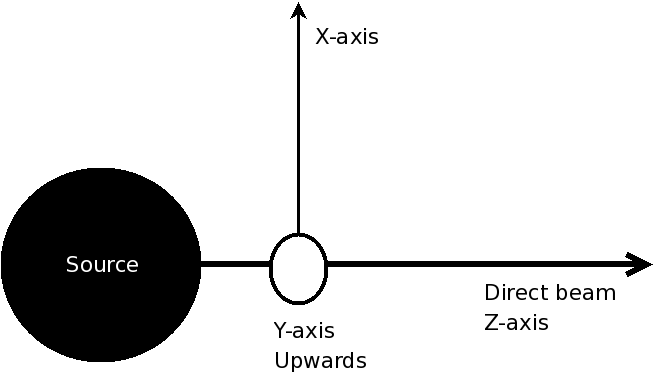
\includegraphics[width=0.75\textwidth]{mcstas.png}}\end{figure}
\end{frame}

\begin{frame} \frametitle{NeXus Simple Coordinate System }
\begin{figure}[!ht]
\resizebox{7cm}{5cm}{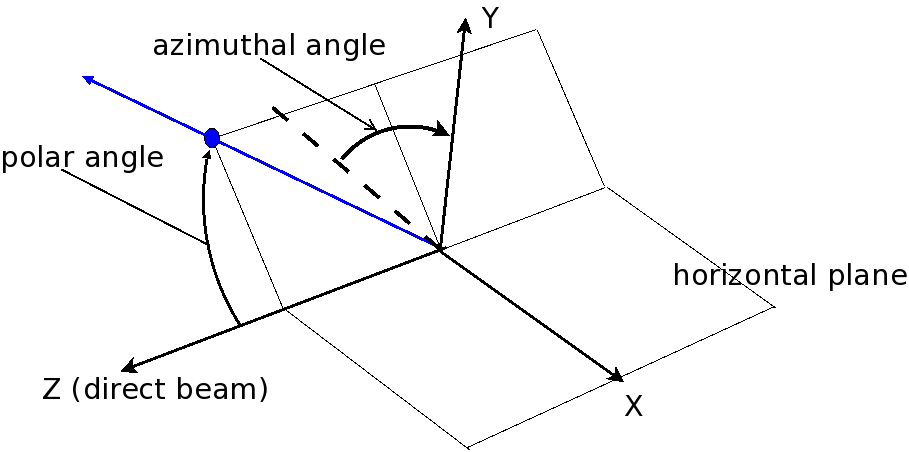
\includegraphics[width=0.75\textwidth]{polplane.png}}\end{figure}
\end{frame}




\begin{frame} 
\frametitle{NeXus Endorsement }
\begin{table}[!ht]
\begin{tabular}{|c|c|c|}
\hline
SNS at ORNL & SINQ at PSI\\ \hline
 NCNR at NIST & ISIS at RAL\\ \hline
 Diamond at RAL&Opal at ANSTO\\ \hline
FRM2 at TUM&KENS at KEK\\ \hline
J-Parc & IPNS at ANL\\ \hline
APS at ANL& HMI in Berlin\\ \hline
MLNSC at LANL& LLB in Saclay\\ \hline
\end{tabular}\end{table}
\end{frame}




\begin{frame} \frametitle{NeXus Levels }
\begin{enumerate}\item Physical file format
\item API for accessing files
\item Structure for organizing data in files
\item Rules for storing individual data items
\item Component and application definitions
\end{enumerate}
\end{frame}

\begin{frame} \frametitle{NXtranslate }
\begin{itemize}\item Anything to NeXus converter:
\begin{itemize}\item Binary dump
\item FRM2
\item IPNS run
\item NeXus
\item Spec
\item XML
\end{itemize}\item Uses XML based translation file to control translation
\item Extendable via plugins
\end{itemize}
\end{frame}

\begin{frame} \frametitle{NXextract}
\begin{itemize}
\item Extracts NeXus files to binary or ASCII
\item Uses XML template file to control conversion
\item Contributed by Stephane Poirier, SOLEIL 
\end{itemize}
\end{frame}


\begin{frame}[fragile] 
\frametitle{Aside: CIF Hierarchies}
CIF uses Hierarchies too, but hides them:
\uncover<1->{
\begin{semiverbatim}
\_exptl\_crystal\_description        plate\newline
\_exptl\_crystal\_colour             colourless\newline
\_exptl\_crystal\_size\_max           0.30
\end{semiverbatim}
}
\uncover<2>{
\begin{semiverbatim}
/exptl/crystal/description        plate\newline
/exptl/crystal/colour             colourless\newline
/exptl/crystal/size/max           0.30
\end{semiverbatim}
}

\end{frame}

\begin{frame}
\frametitle{Why a Common Dataformat? }

\begin{itemize}\item Today: 
\begin{itemize}\item Lots of different data formats
\item Time wasted converting data
\item Old formats no longer capable of delivering for new high throughput detectors
\item Difficult to add additional data
\item Often, for DA multiple different files needed
\item Badly documented formats
\end{itemize}\item Tomorrow, with NeXus:
\begin{itemize}
\item Single, efficient, platform independent data format
\item All information in one file
\item Self describing
\item Extendable
\end{itemize}
\end{itemize}
\end{frame}
